%!TEX root = karulf-thesis.tex
\chapter{Human-Computer Interaction} % (fold)
\label{chapter:hci}
Human-Computer Interaction, HCI, is the study of how humans interface with technology. This includes traditional interfaces, like graphical user interfaces controlled with a mouse and keyboard, as well as alternative interfaces such as the accelerometers in the Nintendo Wii™ controller or the motion tracking system in the Microsoft Kinect™.

Despite the advances in efficacy and popularity of non-traditional devices, the remainder of this paper will be limited to devices standard on most computer systems, e.g., a monitor, mouse, and keyboard. In Section~\ref{section:futurework} I will briefly introduce where alternative interfaces would enhance our proposed interface.

\section{Video Game Interfaces} % (fold)
\label{sec:video_game_interfaces}
Originally created as an application of computer graphics for use in the entertainment industry, video game development has matured into an independent industry in its own right. The popularity of video games has grown significantly throughout the past decade. The Entertainment Software Association estimates 68\% of American households now play computer or video games. \cite{ESA} This large demographic represents a pool of users already versed in exploring 3D virtual worlds interactively. In these interactions users are not only perceiving the a virtual world through simulated senses, but users are also performing actions and controlling their presence in this world through input devices, eg., a mouse and keyboard.

\subsection{Video Games in Research} % (fold)
\label{sub:video_games_in_research}
Due to their common ancestry with human-computer interaction, many of the principals of video game design can be applied to human-robot interaction. There are several published applications of video games to the fields of artificial intelligence and machine learning. We will explore two applications that leverage human resources to compliment artificial intelligence.

Dr. Luis Von Ahn found that video games can be an effective tool for generating training data sets for machine learning. \cite{GWAP} Dr. Von Ahn developed special video games he calls ``games with a purpose''.  These games provide a way to solve problems that may be considered trivial for humans, yet are very challenging for computers. In these games the interaction of the human and the computer has changed to include the human in the computation of data. This is an interesting inversion of traditional autonomy, where the human is given tasks by the computer's artificial intelligence.

% Does GWAP need a "for example" like ESP Game

Dr. Daniel Grollman, in his dissertation work, applied a video games interface with HRI principles to capture training data for robotic user interfaces. \cite{Grollman} Grollman's application, RGame, recorded user’s actions as they controlled a robotic dog and taught it to play soccer. Dr. Grollman was able to create an AI model for shooting and defending using the aggregate of data collected from RGame. Similar to Dr. Von Ahn's research, the RGame interface allowed the computer request information from the user to help it solve a problem.
% subsection video_games_in_research (end)

\subsection{First-Person Games} % (fold)
\label{sub:first_person_games}

% subsection first_person_games (end)

\subsection{Real-Time Strategy Games} % (fold)
\label{sub:RTS_games}

RTS games are full genre in the world of computer and video games. The goal of real-time strategy games is to effectively control your units to achieve a specified goal. Often these goals require the user to control units across a large  map. Real-time strategy games stress a users ability coordinate large numbers of units in a short amount of time. 

RTS games use an isomorphic top-down view to display a large section of the environment at a time. The map can be navigated using either the keyboard or the mouse. Placing the moue pointer on the edge of the screen will translate the camera in the given direction. The keyboard can also be used directly manipulate the camera through both translation and rotation. An example user interface for a simple real time strategy can be seen in Figure ??. 

The control scheme for RTS games is a ``point and click'' style. The player begins by selecting a unit by left clicking on a unit in the viewport. Internally the RTS game uses ray projection to determine which selectable object, if any, was selected. The user interface state is updated to denote a selected unit by updating the on-screen user interface components and marking the unit in the viewport. If the selected action requires a location as an argument, the same ray-tracing technique is used to determine the target location.

% subsection real_time_strategy_games (end)
% section video_game_interfaces (end)


\section{Human-Robot Interaction}
Human-Robot Interaction is a subset of Human-Computer Interaction which focuses on how humans interface with robots. In his survey paper on HRI, Dr. Michael Goodrich introduces five attributes, shown in Figure~\ref{fig:five-attributes} that define the interactions between humans and robots (Goodrich 216-217).

\begin{figure}[ht]
	\makebox[\textwidth]{\hrulefill}
	\begin{list}{$\bullet$}
		\item Level of behavior and autonomy
		\item Nature of information exchange
		\item Structure of the team
		\item Adaptation, learning, and training of people and the robot
		\item Shape of the task
	\end{list}
	\makebox[\textwidth]{\hrulefill}
	\caption{Five attributes of Human-Robot Interaction \label{fig:five-attributes}}
\end{figure}

In the world of robotics, autonomy is defined as the extent of actions a robot may take independently. One of the core ideas behind RIDE is the idea that autonomy may vary depending on context. The concept of ``sliding autonomy'' is introduced in the Section~\ref{section:autonomy}.

Information exchange simply describes the data that flows between a robot and a human. This description characterizes the amount of data that is passed and how the information is visualized. Much like with autonomy, I propose an interface that adapts the nature of information exchange based on context. In Section~\ref{section:infoexchage} I will introduce our refinements to the existing work in this field.

% TODO: Paragraph on Structure of the team

\subsection{Autonomy}

Autonomy, independent robot behavior, is an important factor in HRI design. The relationship between a robot and a human, as provided through the interface, can be viewed or conceptualized along the lines of a continuum or a scale of autonomy. Teleoperation represents one end of the spectrum, where the robot exhibits no qualities of autonomous behavior. On the other hand, a fully autonomous robot, that ignores human input, represents the other extreme of autonomy. A simple scale of autonomy can be found in Figure~\ref{fig:autonomy}. \cite{Goodrich_Survey}


\begin{figure}[ht]
\begin{center}
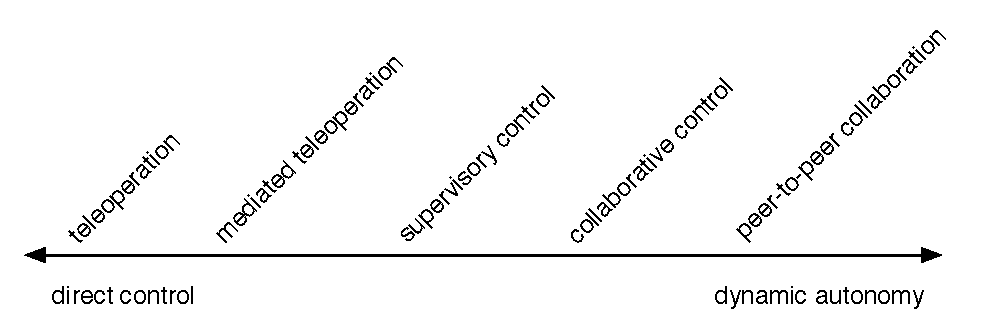
\includegraphics[width=5in]{images/autonomy.pdf}
\caption{Scale of Robot Autonomy\label{fig:autonomy}}
\end{center}
\end{figure}

% Awk. -ek
Robots, as they presently exist, have a fairly limited set of autonomous actions available. As a result, most interfaces, currently, are artificially conservative in their autonomy due to limitations in artificial intelligence. As research into artificial intelligence and machine learning grows, a much more diverse set of autonomous behaviors will inevitably become available. As user interface designers, we are tasked to create extensible interfaces to support future behaviors.

The idea of sliding autonomy allows the human and a robot to change the level of autonomy as needed. For illustration purposes, consider a robot that explores a warehouse. If the robot planned a poor navigation path, a user could manually specify the waypoints of an optimal path. If the robot is unable to complete the specified path due to an obstruction in the path, the robot could ask the user to directly teleoperate around the obstacle. Once free of the obstruction, the user would input a new set of goal coordinates and allow the autonomous navigation system to resume control. When combined with machine learning, sliding autonomy provides the robot a fantastic platform for interactive learning from demonstration. The idea of interactive learning from demonstration is already well established from the RGame project.

\subsection{Information Exchange}
\label{sub:info_exchange}
The nature of information exchange defines the flow of data between the human and the robot. What information is provided, how it is represented, and when it is communicated are all properties of the interface design. This encompasses low-level communication of navigation and sensor data as well as high-level commands sent from the human. 

The purpose of visualization interfaces is to represent the one-way exchange of information from the robot to humans. This data typically includes location information, laser or sonar readings, battery readings, accelerometer readings, and map data. Original interfaces were written to be accessible programatically. These interfaces were slowly adapted to display sensor data graphically, but the resulting interfaces were disjoint and required operator training. Examples of these 2D user interfaces can be seen in Figure~\ref{existing-robot-ui}.

In 2007 Dr. Curtis Nielsen introduced an ecological user interface with the goal of combining sensor data into a single, integrated display. Nielsen designed his interface to for effective teleoperation, the technique of controlling a robot remotely. In his study, Nielsen compared an integrated 3D user interface to a simple 2D user interface for several environment searching tasks. The 3D user interface displayed combined sensor data through a single viewport while the 2D user interface displayed the same data through individually. The study found the 3D interface decreased collisions and decreased task completion time. \cite{Nielsen_Teleoperation}

Nielsen attributes the success of the 3D interface to improved situational awareness. The observed effect of situational awareness and context on interface effectiveness is congruous with the findings of other researchers. \cite{Nielsen_Teleoperation}

A limitation of Nielsen's interface is that it's focus on teleoperation leaves the robot without autonomy. While teleoperation may be optimal for single robot environments it does not allow for concurrent robot control. This limitation requires an human operator for every active robot. We believe that providing an ecological interface common to multiple robots allows for more efficient use of human resources.

\subsection{Prior Work} % (fold)
\label{sub:hri_prior_work}

% subsection prior_work (end)
% chapter hci (end)
